% \documentclass[twocolumn]{article}
\documentclass{article}
\usepackage{graphicx} % Required for inserting images

\usepackage{wrapfig}

\usepackage{caption}
\usepackage{subcaption}


\usepackage{biblatex}
% \usepackage[style=authoryear,sorting=ynt]{biblatex}
\addbibresource{ref.bib}      % kon file er vitor reference ase , setar naam

\usepackage{hyperref}  %  to create reference link like in contents 

\usepackage{multicol}
\usepackage{lipsum} 

\title{CSE 200 Tutorial 2}
\author{Abdur Rafi}
\date{\today}

\begin{document}

\maketitle
\tableofcontents
\listoffigures

\pagebreak

\section{Images}
%% "//" emon kisu nai in latex . Rather use '\\' for newlines .Also here '\' for division sign
\subsection{Basic Image}


\includegraphics{Images/CSE_BUET.png}

\pagebreak


\subsection{Image Size}

\subsubsection{Fixed Size} 
 % to insert the image. also u can specify height or width inside 3rd bracket

\includegraphics[width=6cm]{Images/CSE_BUET.png}   \\ % add this thing MUST ! naile new line e jabena image ta.       
      

\includegraphics[width=6cm, height=4cm]{Images/CSE_BUET.png}


\pagebreak


\subsubsection{Scaling}

\includegraphics[scale=.2]{Images/CSE_BUET.png}

\includegraphics[scale=1.2]{Images/CSE_BUET.png}

\pagebreak

\subsubsection{Relative to document}
                    % VERY VERY IMPORTANT

\includegraphics[width=.5\textwidth]{Images/CSE_BUET.png}

\pagebreak

\subsection{Rotation}

\includegraphics[scale=.5,angle=45]{Images/CSE_BUET.png}

\pagebreak

\subsection{Positioning, Alignment and Caption }  % VERY VERY IMPORTANT

\subsubsection{Positioning}

\begin{figure}[htbp]
    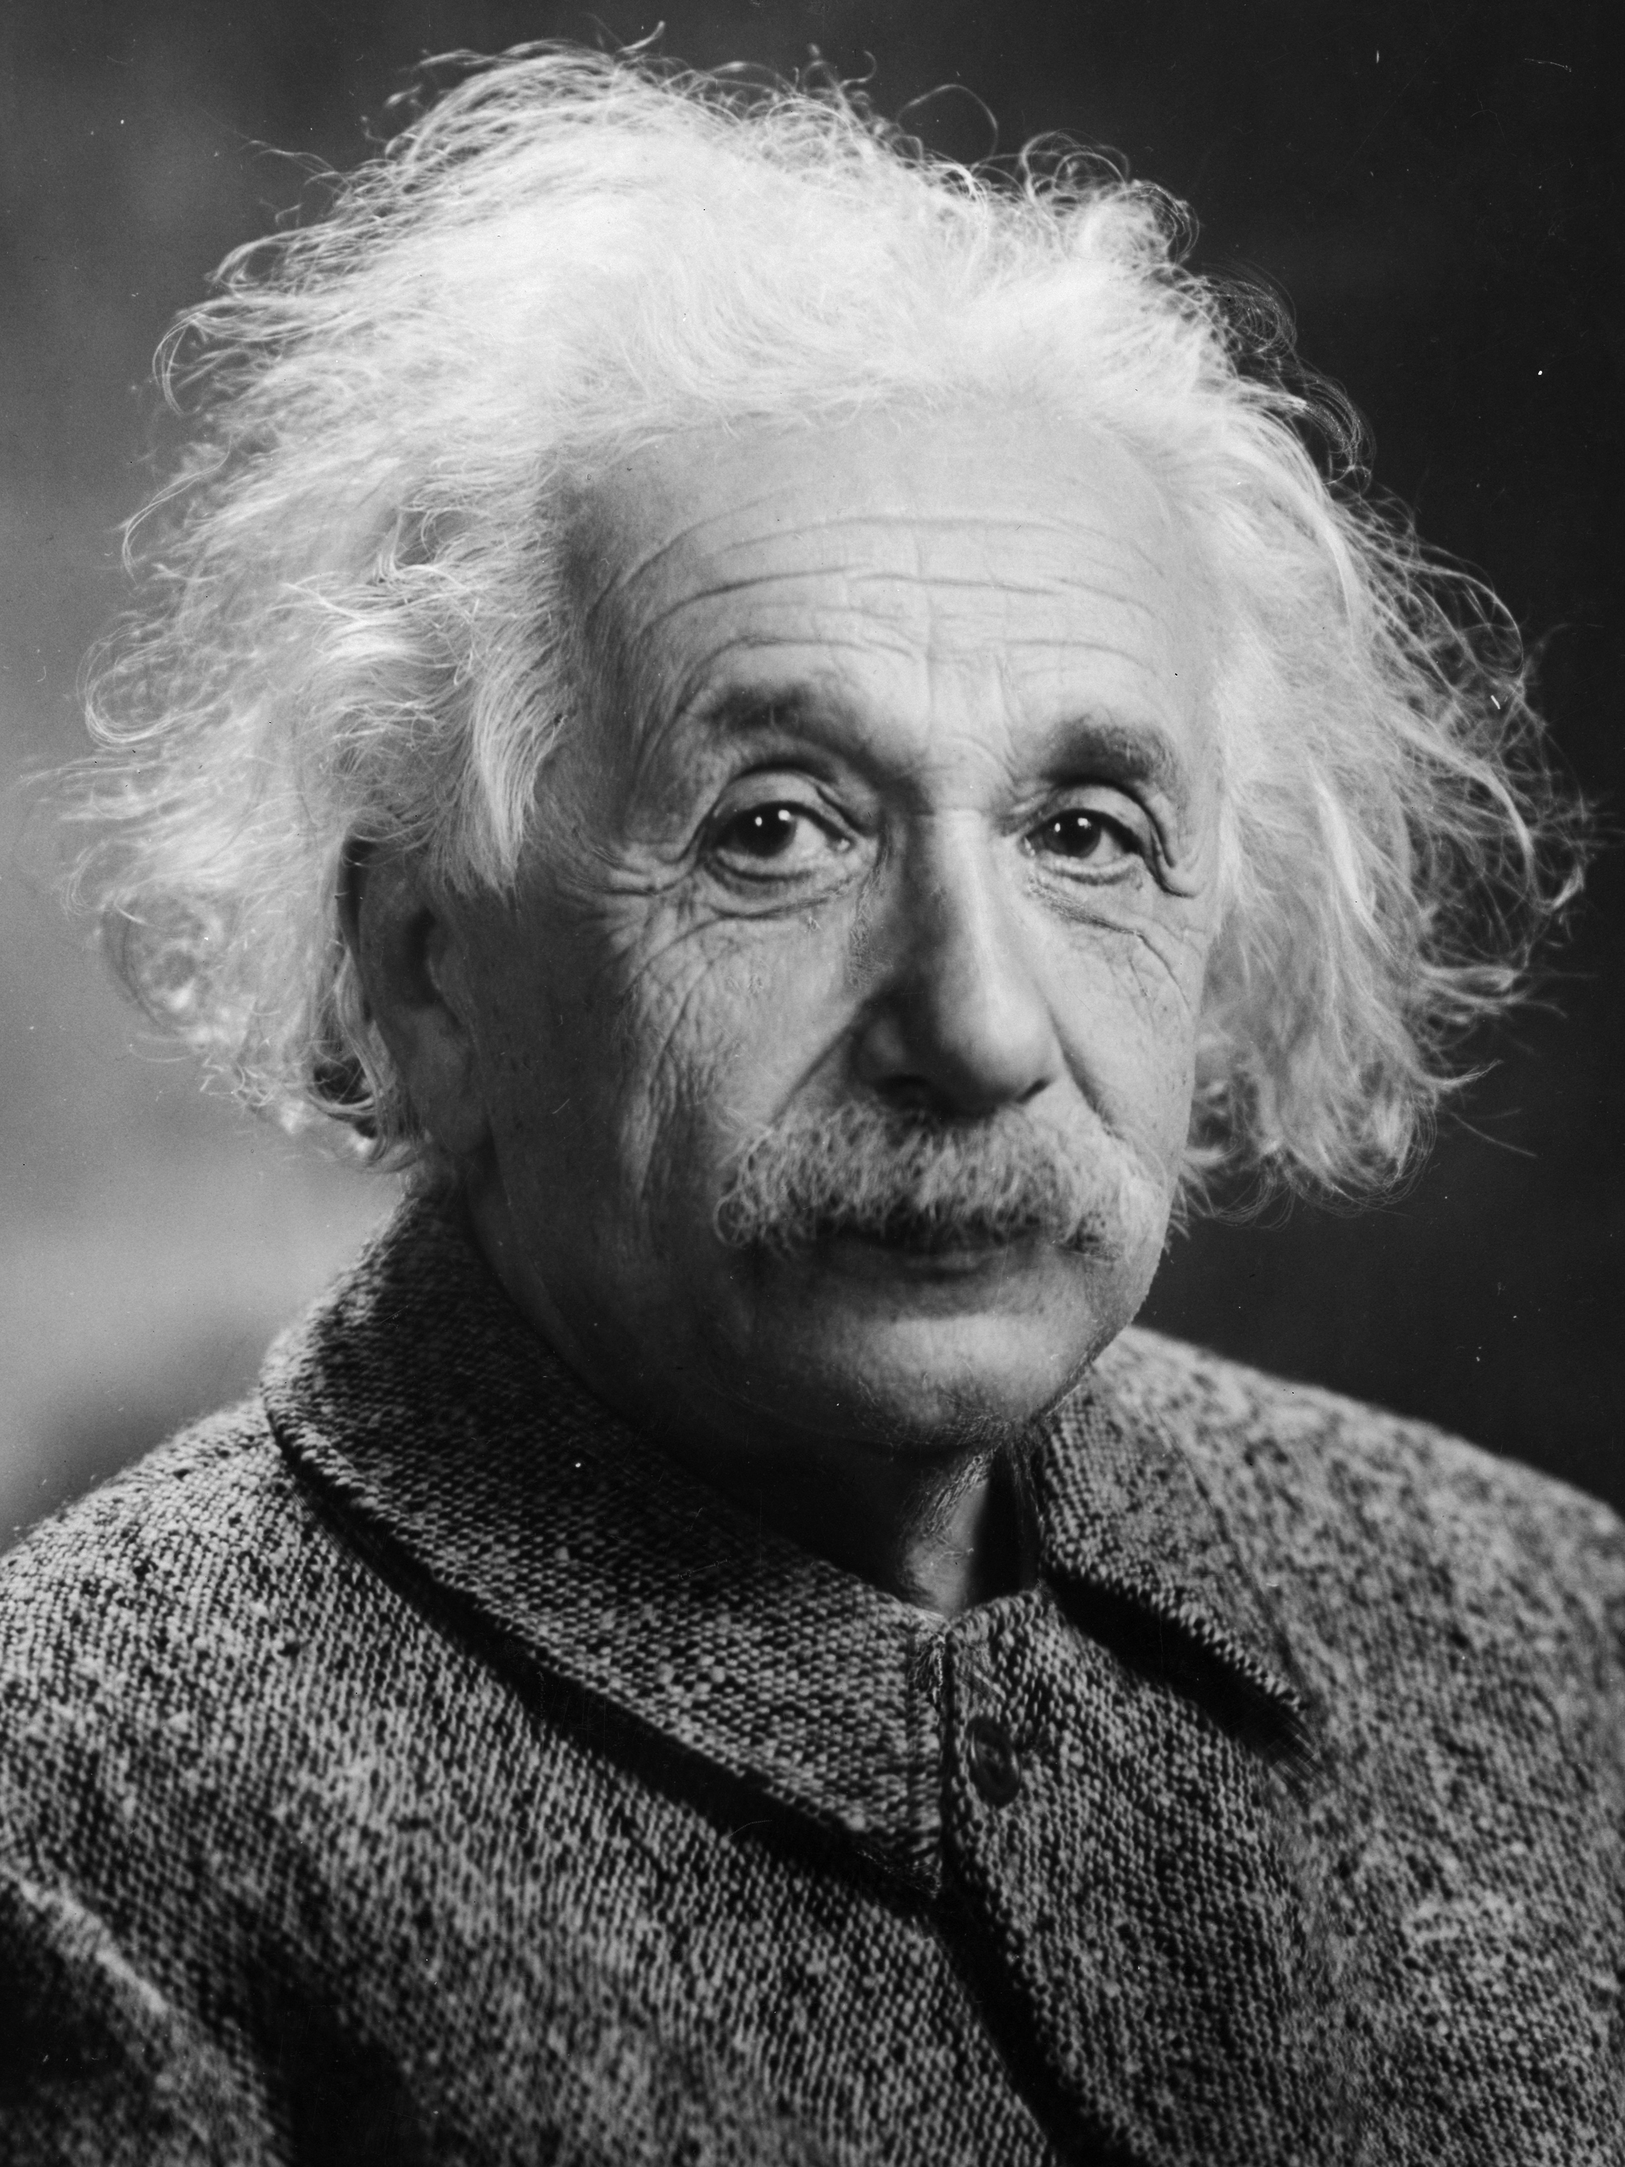
\includegraphics{Images/Albert_Einstein.png}
    \caption{Positioned and Left Aligned Image}
\end{figure}

\pagebreak

\subsubsection{Center Alignment}
\begin{figure}[htbp]
    \centering
    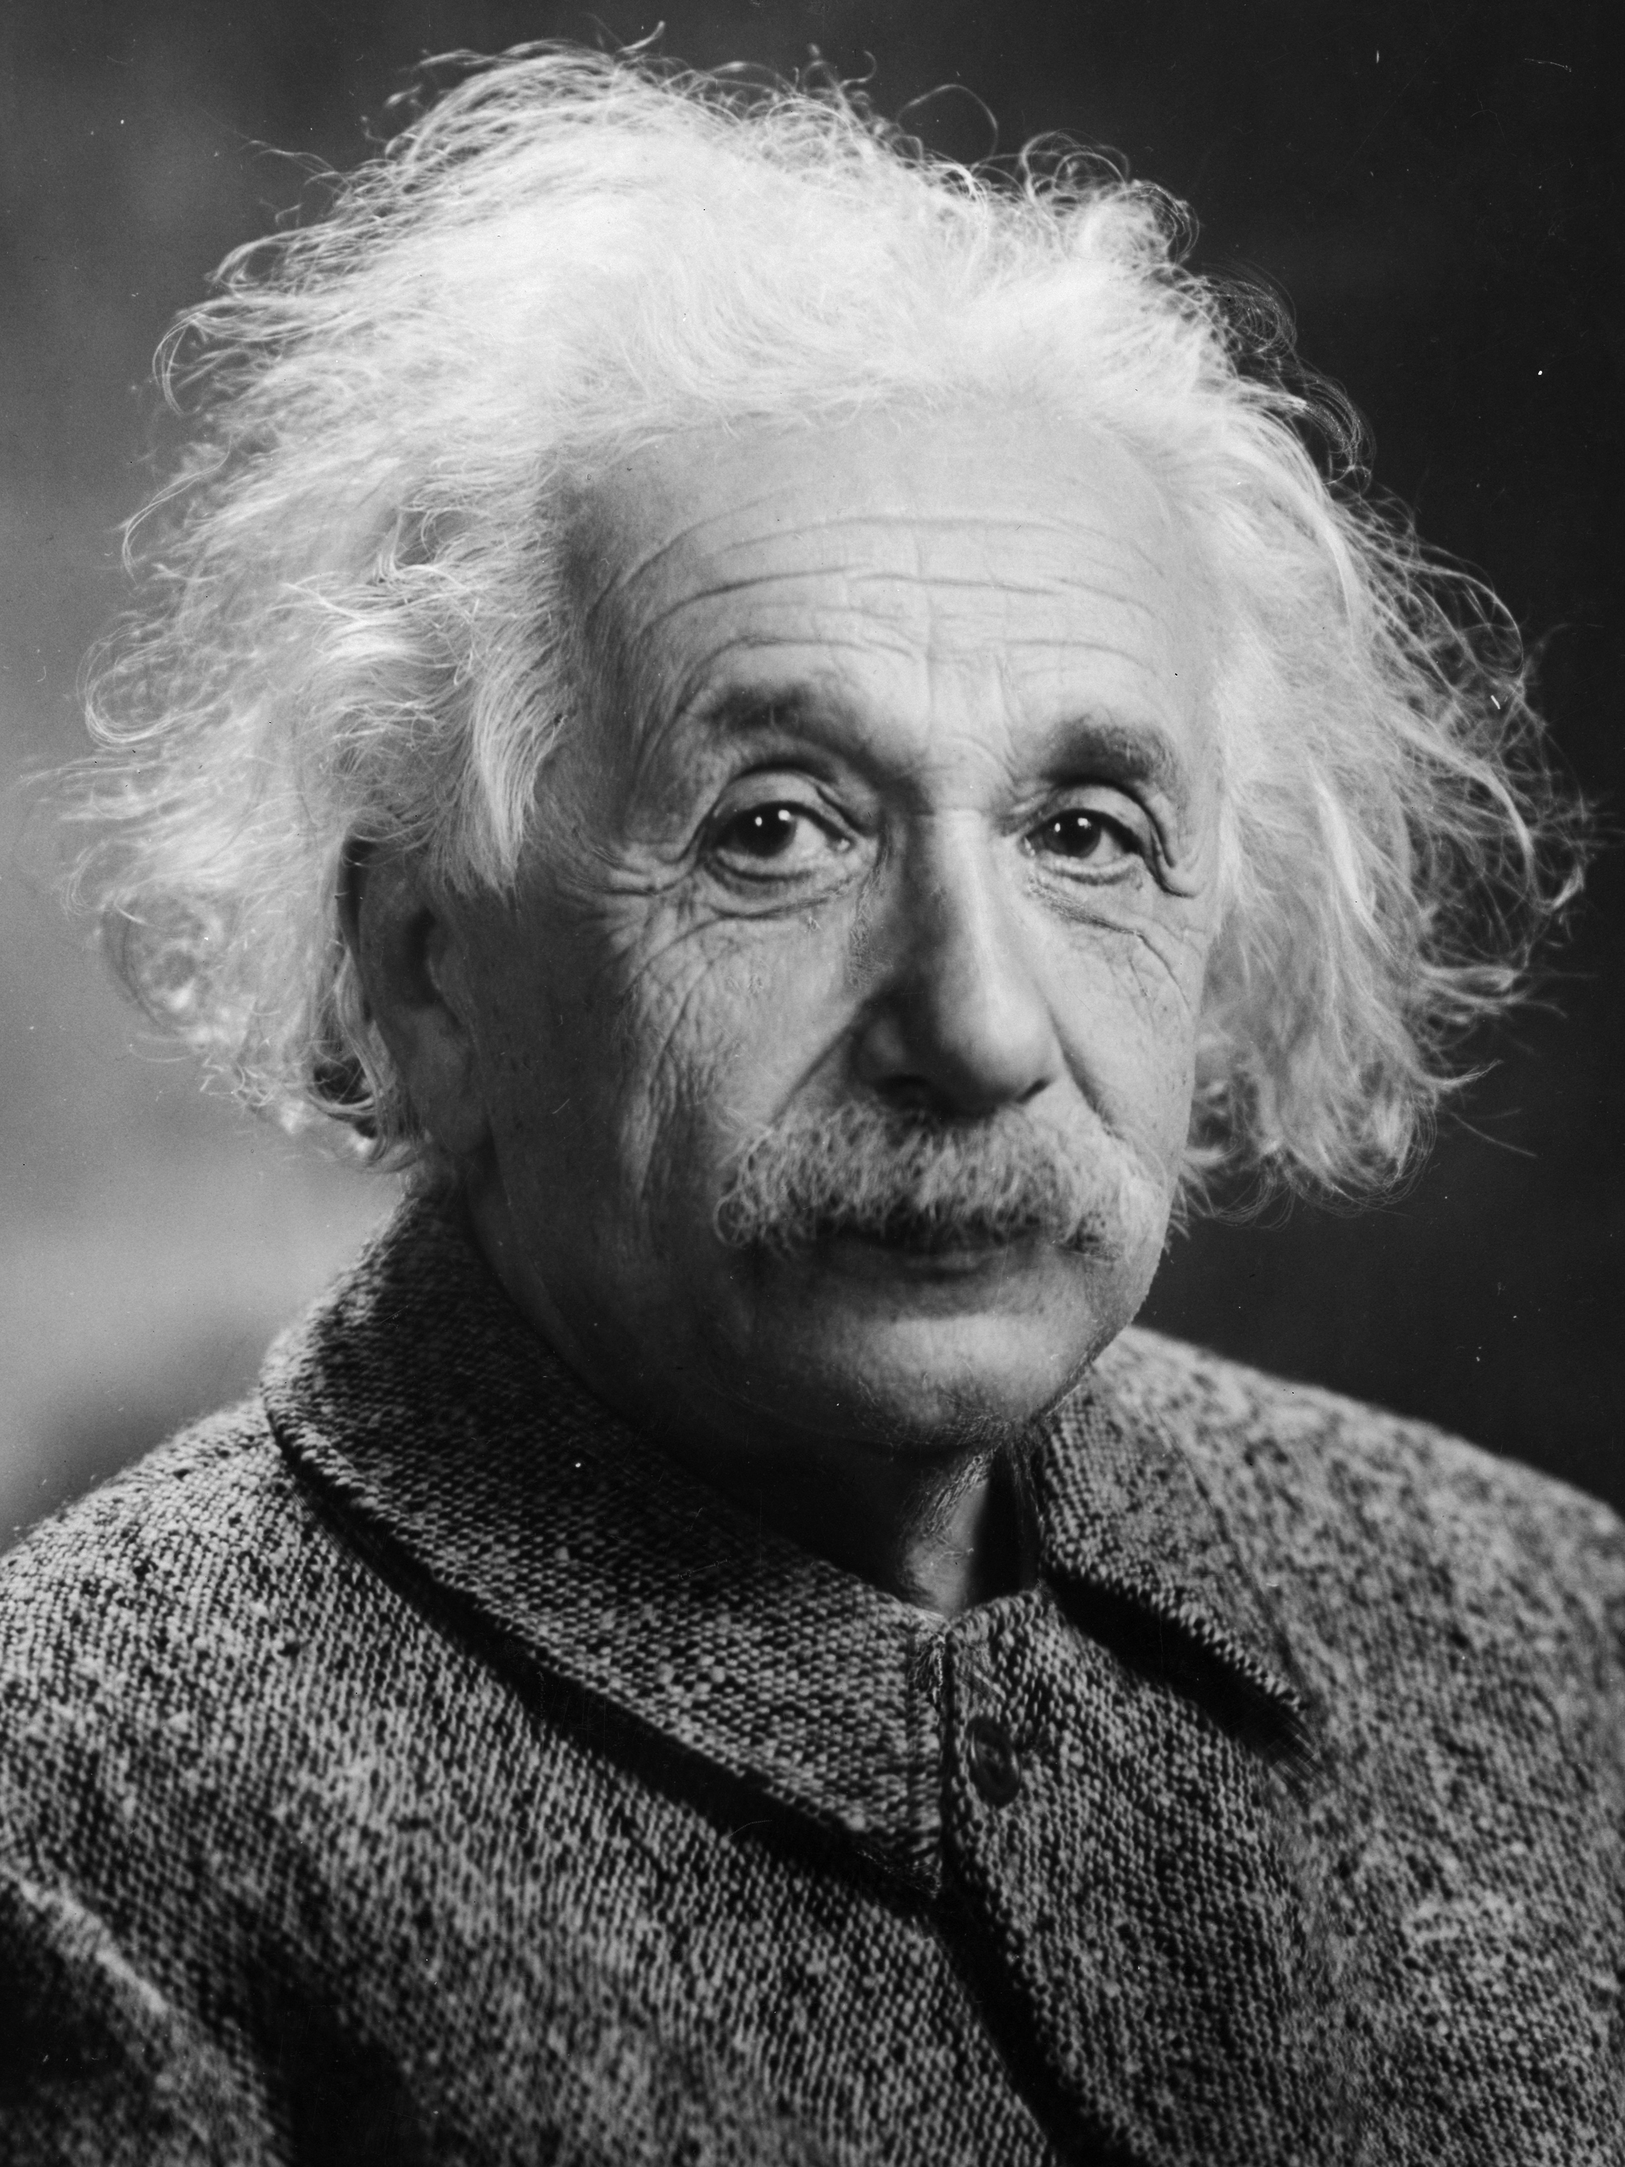
\includegraphics{Images/Albert_Einstein.png}
    \caption{Center Aligned Image}
\end{figure}
\pagebreak

\subsubsection{Right Alignment}
\begin{figure}[htbp]
    \hfill      %%  need to write this for right align
    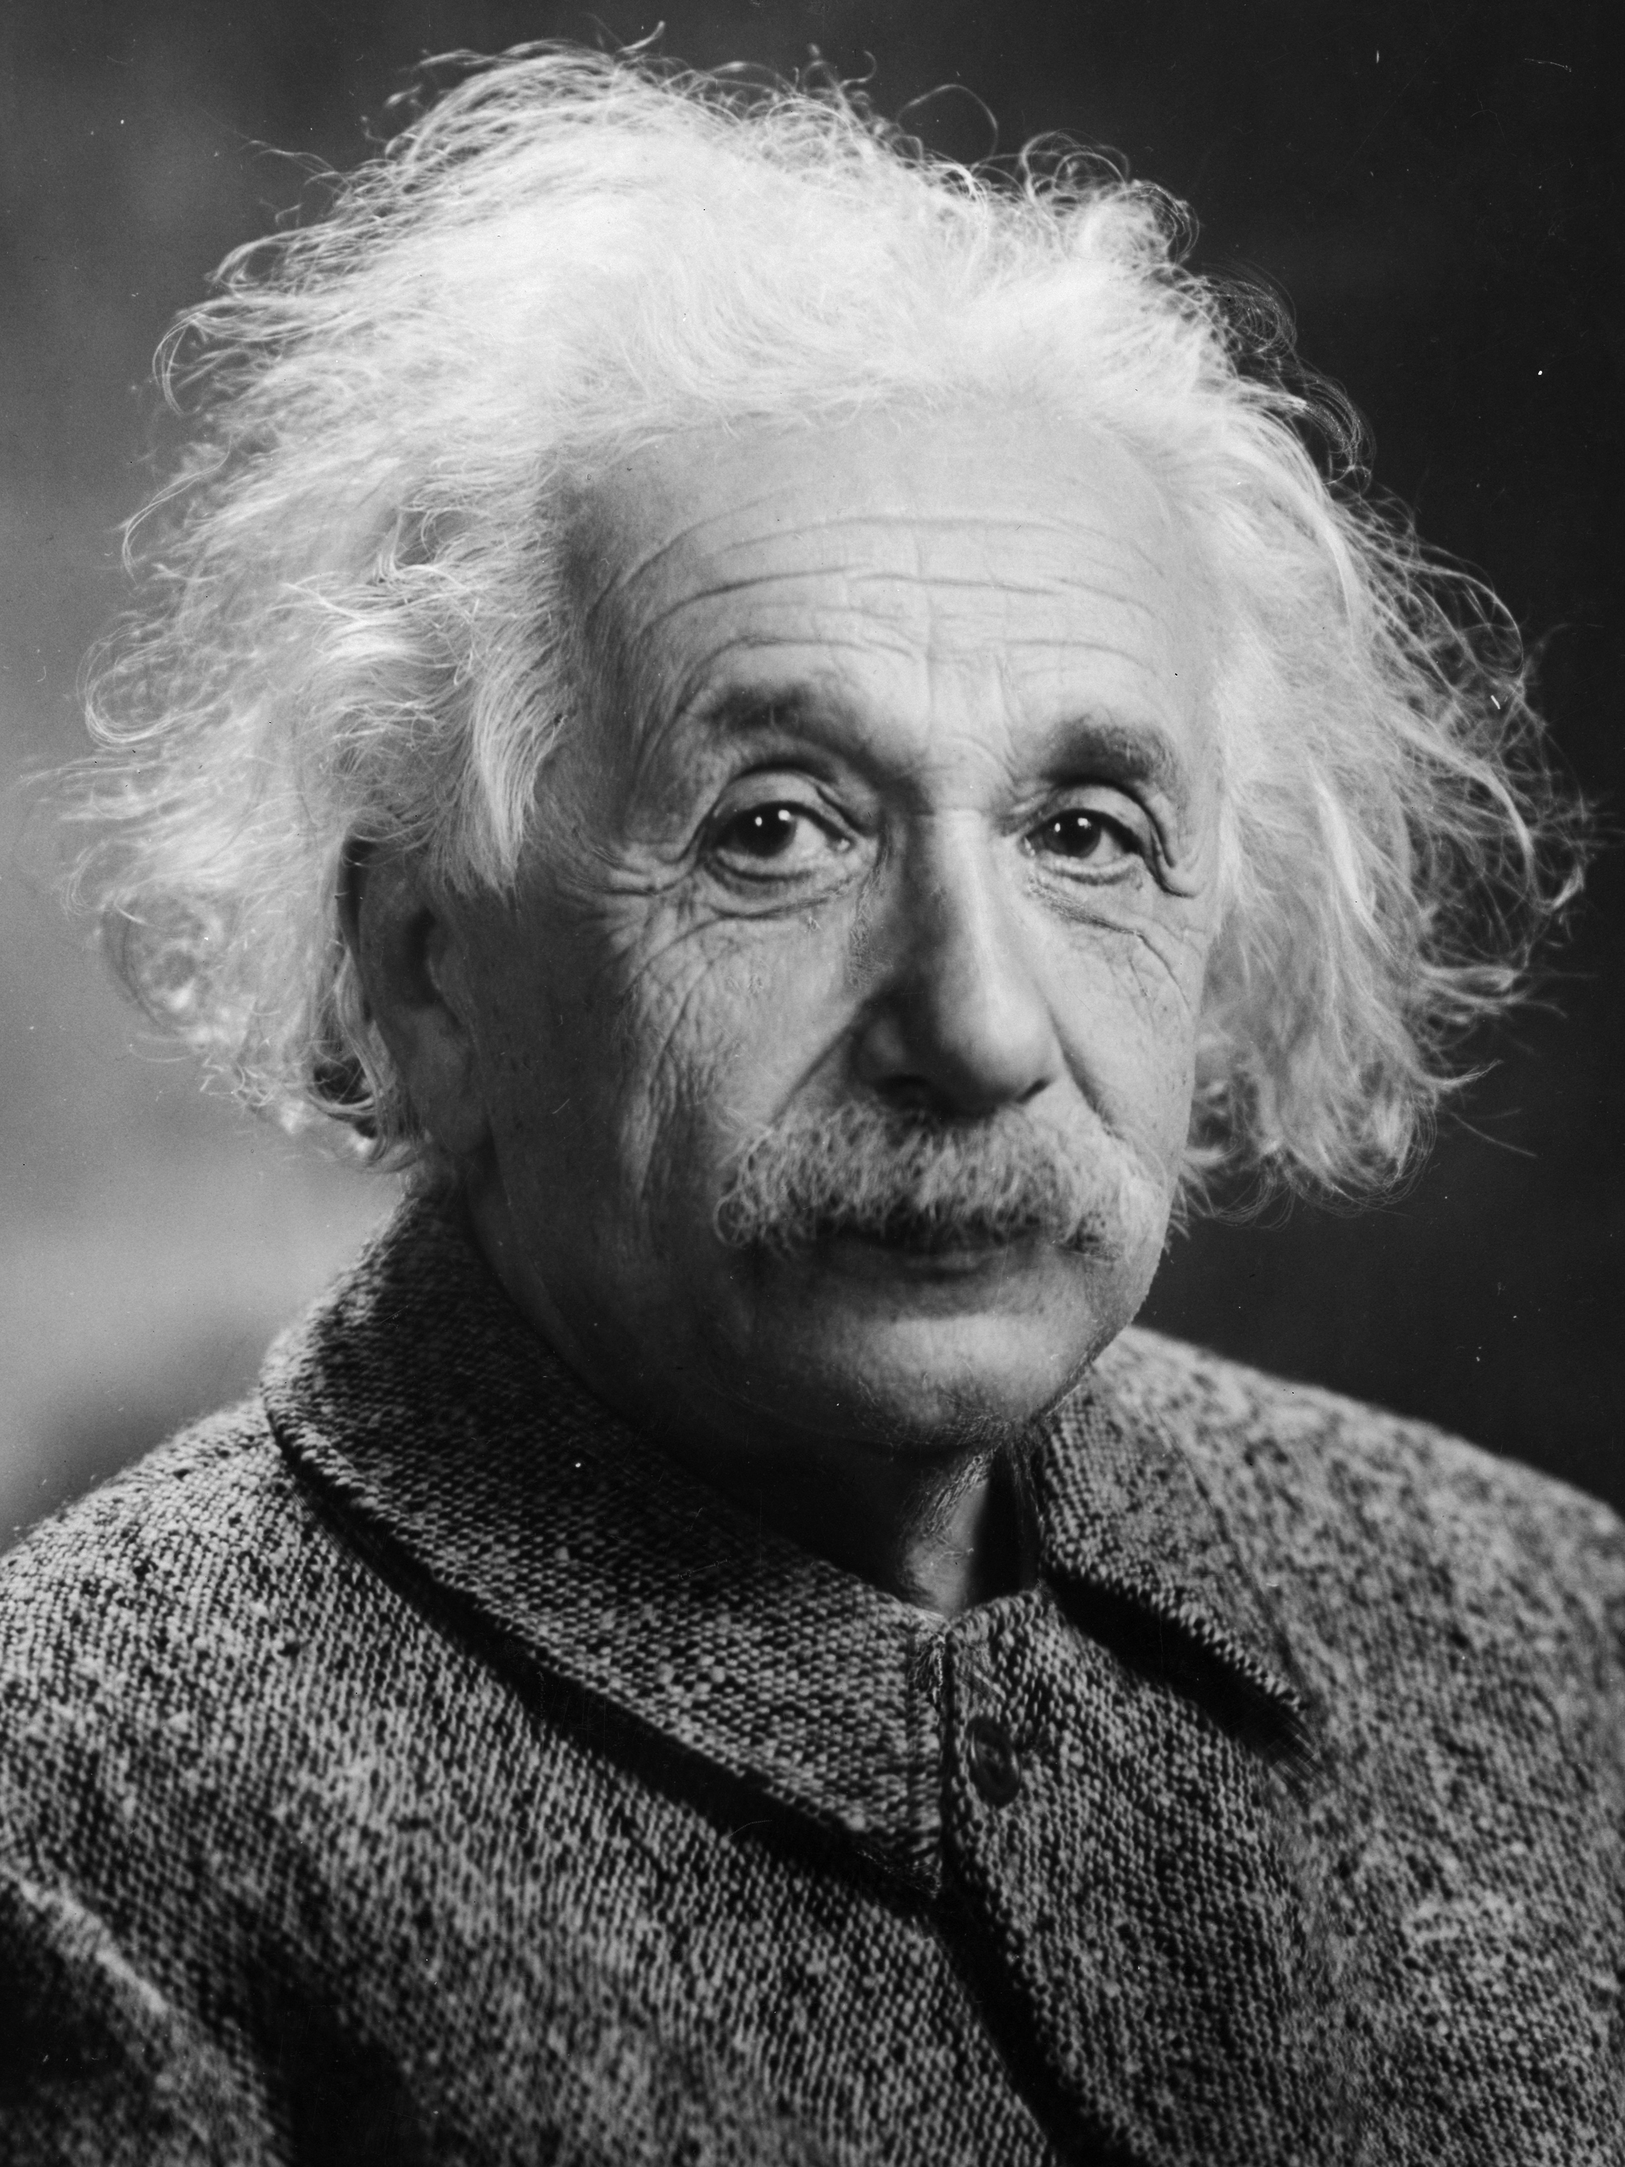
\includegraphics[]{Images/Albert_Einstein.png}
    \caption{Right Aligned Image}
    \label{fig:enter-label}
\end{figure}
\pagebreak


\subsubsection{Wrap Text Around Figures}
  % small image r ekdom pashapashi text thakbe which looks nicer ! usepackage 'wrapfigure'
\begin{wrapfigure}{r}{0.25\textwidth}  %% r for 'right'
    \centering
    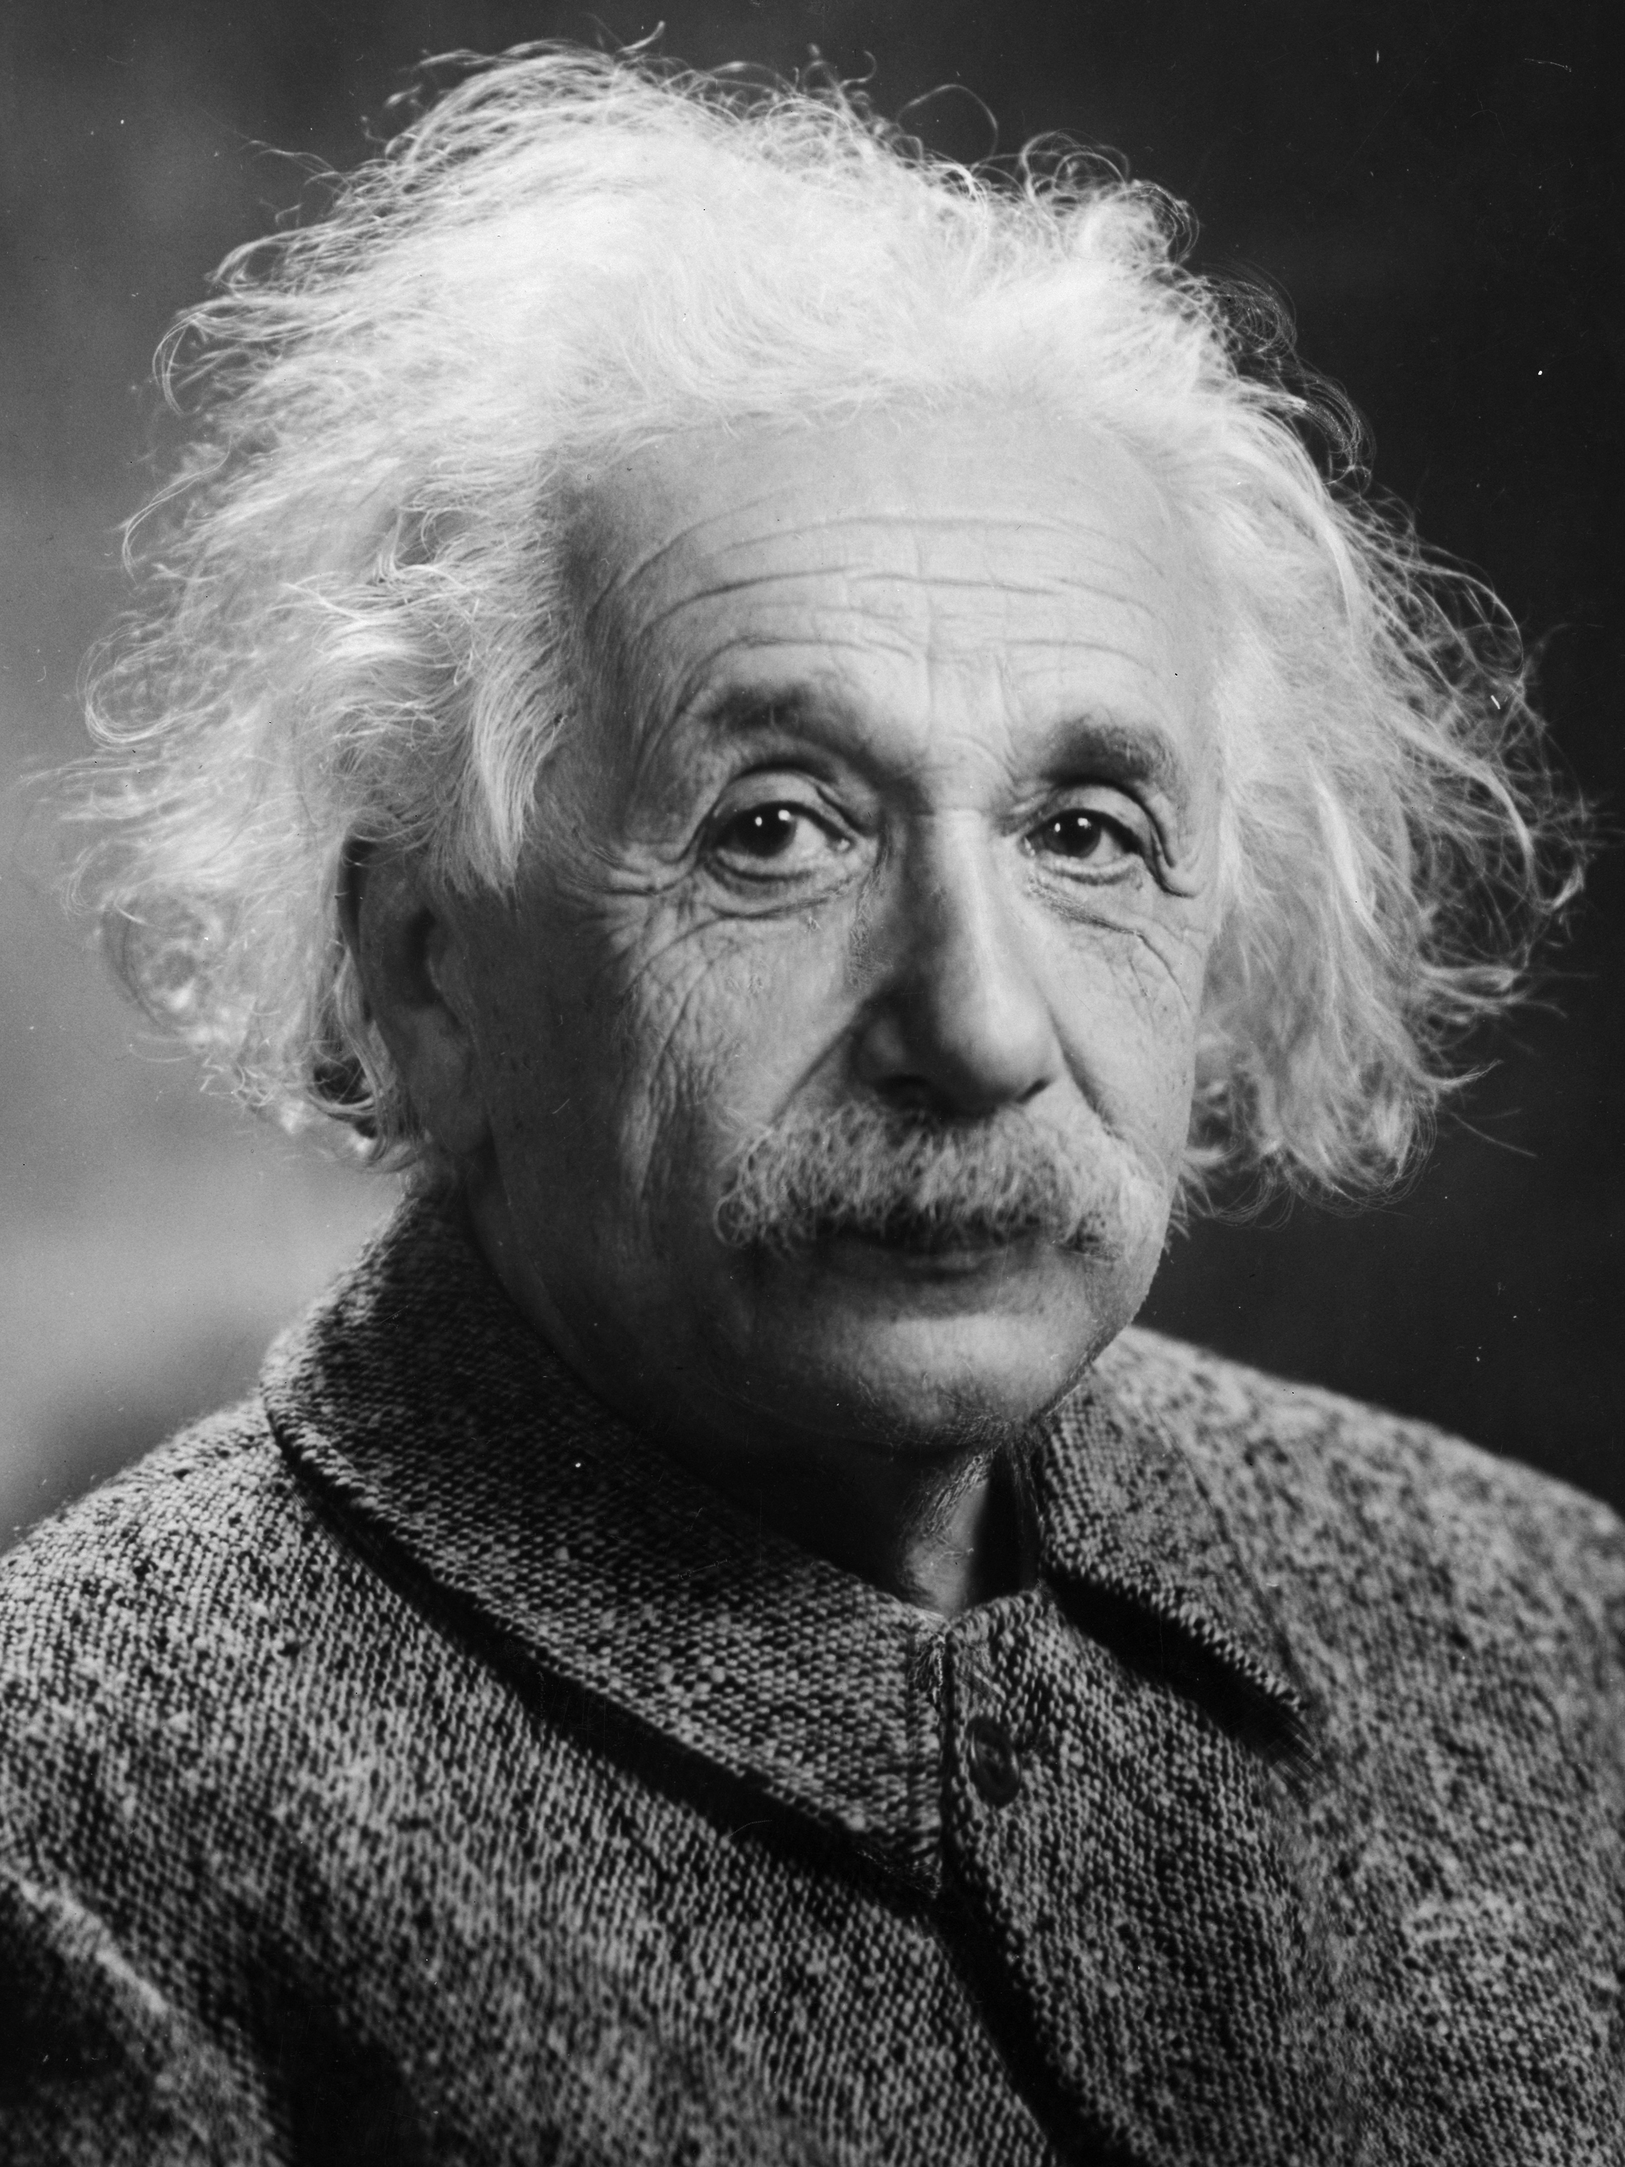
\includegraphics[width=0.25\textwidth]{Images/Albert_Einstein.png}
\end{wrapfigure}

Lorem Ipsum is simply dummy text of the printing and typesetting industry. Lorem Ipsum has been the industry's standard dummy text ever since the 1500s, when an unknown printer took a galley of type and scrambled it to make a type specimen book. It has survived not only five centuries, but also the leap into electronic typesetting, remaining essentially unchanged. It was popularised in the 1960s with the release of Letraset sheets containing Lorem Ipsum passages, and more recently with desktop publishing software like Aldus PageMaker including versions of Lorem Ipsum.

\pagebreak


\subsection{Subplots}
\subsubsection{In A Row}
\begin{figure}[htbp]
     \centering
     \begin{subfigure}{0.3\textwidth}
         \centering
         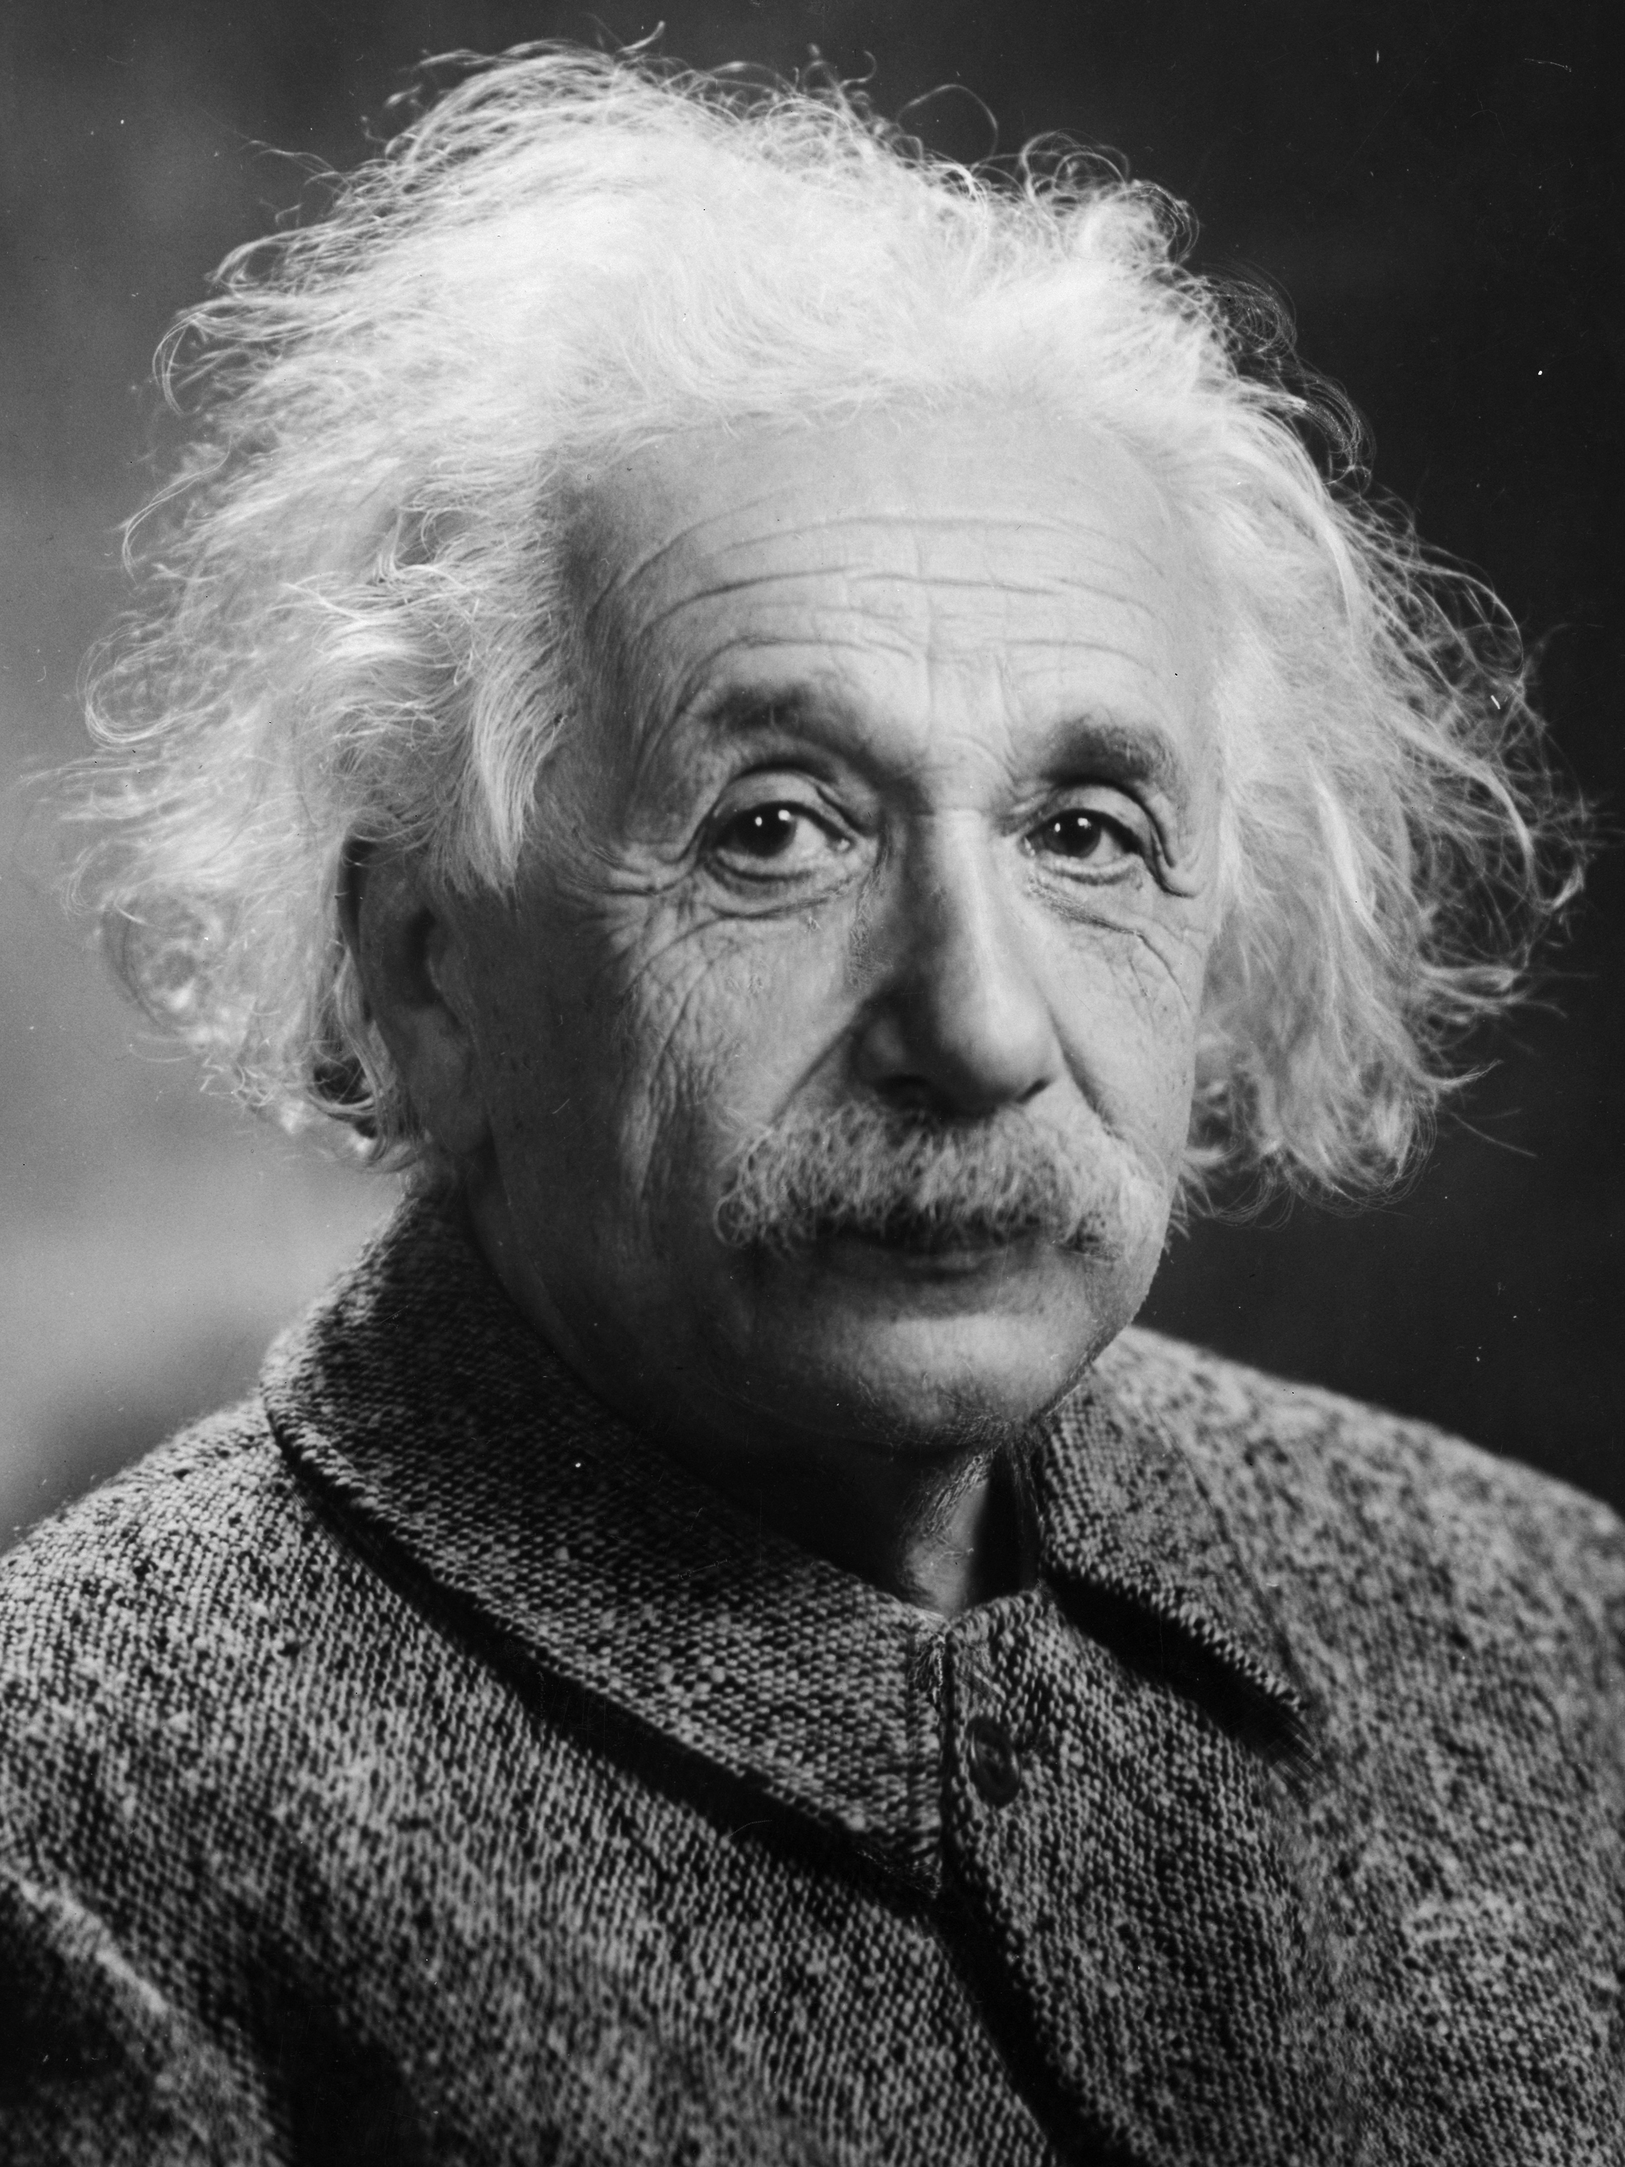
\includegraphics[width=\textwidth]{Images/Albert_Einstein.png}
         \caption{Image 1}
     \end{subfigure}
     \hfill
     \begin{subfigure}{0.3\textwidth}
         \centering
         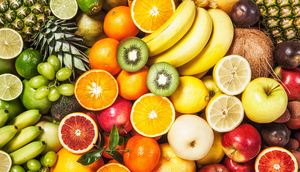
\includegraphics[width=\textwidth]{Images/Fruits.png}
         \caption{Image 2}
     \end{subfigure}
     \hfill
     \begin{subfigure}{0.3\textwidth}
         \centering
         
\includegraphics[width=\textwidth]{Images/CSE_BUET.png}
         \caption{Image 3}
     \end{subfigure}
        \caption{Three Images}
\end{figure}

\pagebreak

\subsubsection{In Multiple Rows}

\begin{figure}[htbp]
     \centering
     \begin{subfigure}{0.45\textwidth}
         \centering
         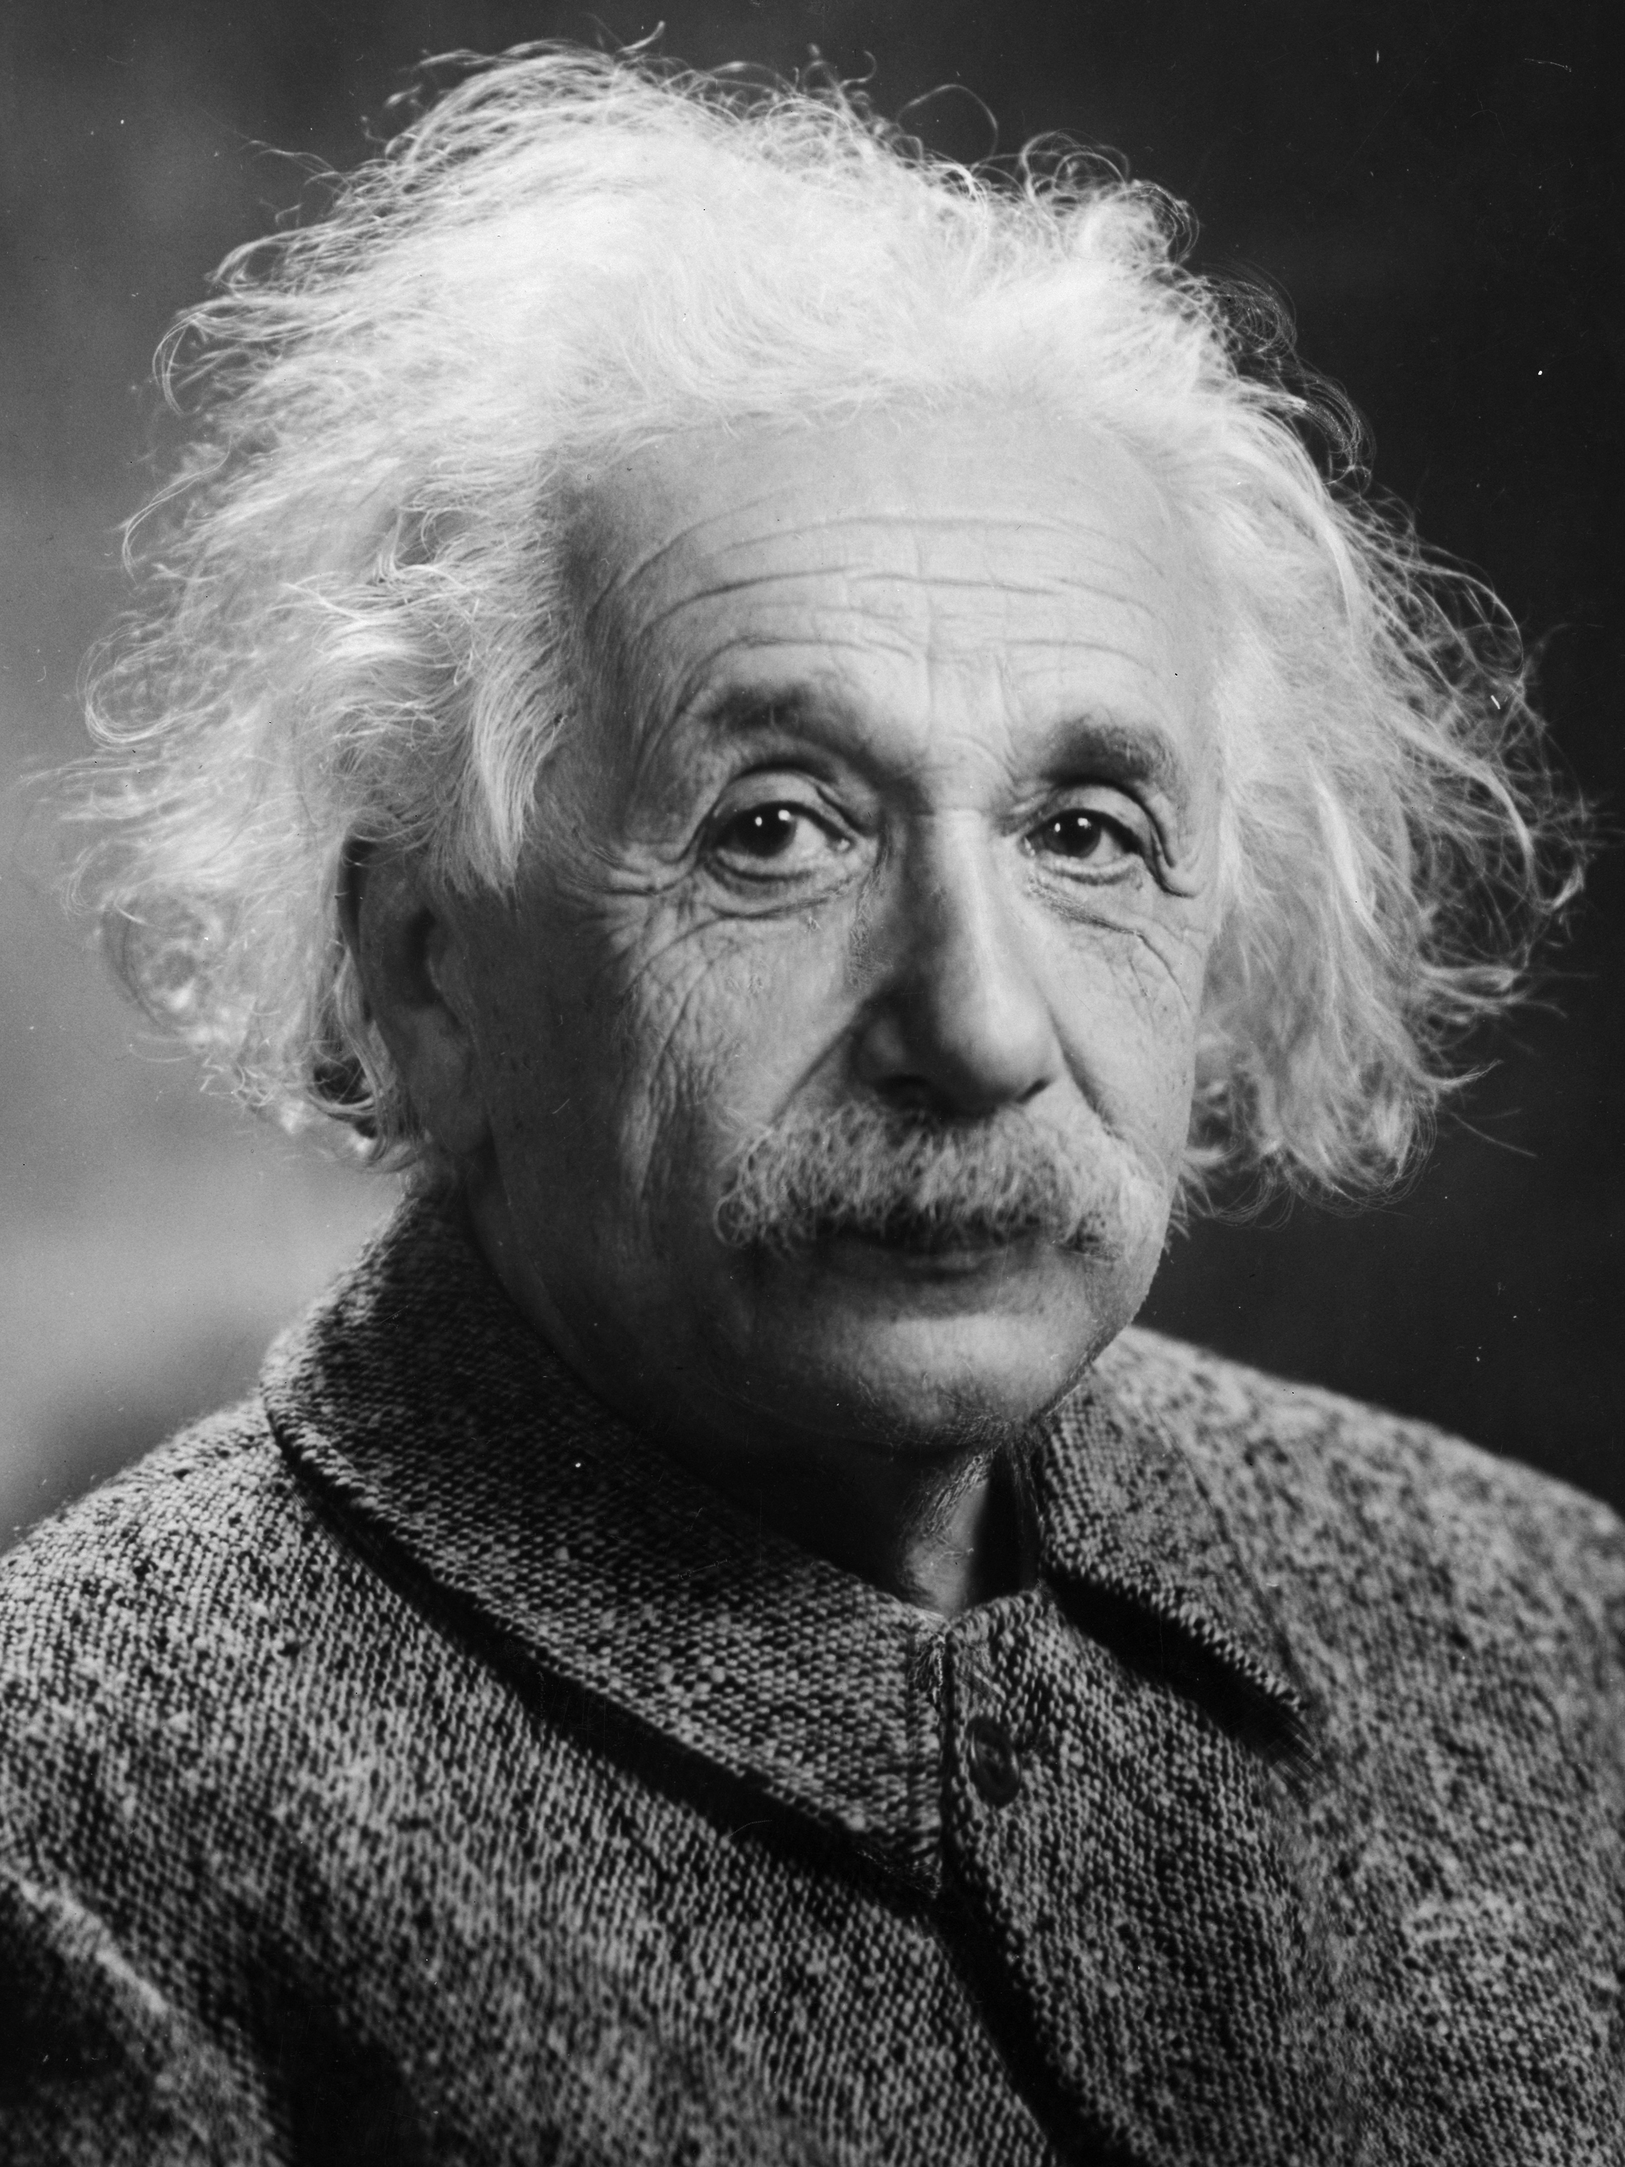
\includegraphics[width=\textwidth]{Images/Albert_Einstein.png}
         \caption{Image 1}
         \label{fig:1}
     \end{subfigure}
     \hfill
     \begin{subfigure}{0.4\textwidth}
         \centering
         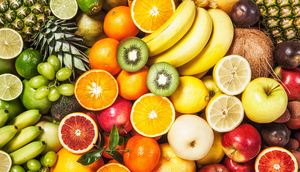
\includegraphics[width=\textwidth]{Images/Fruits.png}
         \caption{Image 2}
         \label{fig:2}
     \end{subfigure}
     \hfill
     \begin{subfigure}{0.6\textwidth}
         \centering
         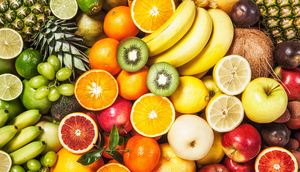
\includegraphics[width=\textwidth]{Images/Fruits.png}
         \caption{Image 3}
         \label{fig:3}
     \end{subfigure}
     \hfill
     \begin{subfigure}{0.3\textwidth}
         \centering
         
\includegraphics[width=\textwidth]{Images/CSE_BUET.png}
         \caption{Image 4}
         \label{fig:4}
     \end{subfigure}
     
        \caption{Three Images}
        \label{fig:4 graphs}
\end{figure}

\section{Multi Column}
\begin{multicols}{2}  
% need package forthis \multicols. WRITE this in main.tex file
\subsection{First Subsection}
Contrary to popular belief, Lorem Ipsum is not simply random text. It has roots in a piece of classical Latin literature from 45 BC, making it over 2000 years old. Richard McClintock, a Latin professor at Hampden-Sydney College in Virginia, looked up one of the more obscure Latin words, consectetur, from a Lorem Ipsum passage, and going through the cites of the word in classical literature, discovered the undoubtable source. Lorem Ipsum comes from sections 1.10.32 and 1.10.33 of "de Finibus Bonorum et Malorum" (The Extremes of Good and Evil) by Cicero, written in 45 BC. This book is a treatise on the theory of ethics, very popular during the Renaissance. The first line of Lorem Ipsum, "Lorem ipsum dolor sit amet..", comes from a line in section 1.10.32.
\subsection{Second Subsection}
Contrary to popular belief, Lorem Ipsum is not simply random text. It has roots in a piece of classical Latin literature from 45 BC, making it over 2000 years old. Richard McClintock, a Latin professor at Hampden-Sydney College in Virginia, looked up one of the more obscure Latin words, consectetur, from a Lorem Ipsum passage, and going through the cites of the word in classical literature, discovered the undoubtable source. Lorem Ipsum comes from sections 1.10.32 and 1.10.33 of "de Finibus Bonorum et Malorum" (The Extremes of Good and Evil) by Cicero, written in 45 BC. This book is a treatise on the theory of ethics, very popular during the Renaissance. The first line of Lorem Ipsum, "Lorem ipsum dolor sit amet..", comes from a line in section 1.10.32.


\end{multicols}


% add necessary packages
% Also if use multi coln, then in case of images, replace 'textwidth' with 'columnwidth'



\section{Referencing In Latex}
% FOrmat - 01 -- witout using any extra package. Also comment out biblatex package 1st. it will show no of reference. Main prob is - we cant customize the numbering. so better to use 'biblatex' package.

    %I am citing \cite{lamport94}     %UNCOMMENT OUT this and comment out biblatex packages to see the use of bibitem and thebibliography parts !!
    % \begin{thebibliography}{9}
    
    % \bibitem{texbook}  % name of the reference item and then in details
    % Donald E. Knuth (1986) \emph{The \TeX{} Book}, Addison-Wesley Professional.
    
    % \bibitem{lamport94}
    % Leslie Lamport (1994) \emph{\LaTeX: a document preparation system}, Addison
    % Wesley, Massachusetts, 2nd ed.
    
    % \end{thebibliography}

    
% part of biblatex package.. jei jei reference use korsi only segula show korbe in document.

% format - 02
I am citing \cite{einstein}.  \\
Here are some info that I got from this \cite{astral_pro_2}. \\
Check out this \cite{latexcompanion} to learn more

\printbibliography  %% WRITE IT !

\begin{figure}[p]
    \centering
    
\includegraphics[width=0.9\linewidth]{image.png}
    \caption{Enter Caption}
    \label{fig:enter-label}
\end{figure}

\end{document}

% READ THIS !!

% cant customize referencing jemon 1 2 evabe ashe reference by default.also reference use hok ba na hok shb reference sec e thake what if only jei reference use kri segula visible holo?wsste of space... for all these solving, so usepackage{biblatex} and add bibresource{} . it will create a new bib file with all references.also write usepackage[style=year, sorting-=ynt]{} add these for replace 1 2 3 with some texts .

% ekta file r upor onk manush eksath kaj krle problem ase..to solve it, use /include{multicol.tex} or /input{multicol.tex} . 2nd cmmand is better bcz oita onner file r content ke copy paste kre dey jaegamoto..1st cmd te new page e kore. 

% usepackage{multicoln} for multiple coln in one space..pasahpasi onkgula diff paragapragh

% use columnwidth instead of textwidth but when !? subfig gula kete jae onk somoy

% onner file r ja packaage shb ekta main DOCUment file r shuru tei sudu DITE HBE !
    
% read  documentation ase for thesis writing in overleaf
